\listfiles

\documentclass[12pt,a4paper,titlepage]{article}

\usepackage[utf8]{inputenc}
\usepackage[T1]{fontenc}
\usepackage[english]{babel}
\usepackage{xpatch}
\usepackage{babel}
\usepackage{titlesec}
\usepackage{csquotes} 
\usepackage{filecontents}
\usepackage[style=authoryear,maxcitenames=2,backend=bibtex]{biblatex}
\usepackage{tabulary}
\usepackage{tabularx}
\usepackage{lscape}
\usepackage{rotating}
\usepackage{longtable}


% Pretty much all of the ams maths packages
\usepackage{amsmath,amsthm,amssymb,amsfonts}
% Allows you to manipulate the page a bit
\usepackage[a4paper]{geometry}
% Pulls the page out a bit - makes it look better (in my opinion)
\usepackage{a4wide}
% Removes paragraph indentation (not needed most of the time now)
\usepackage{parskip}
% Allows inclusion of graphics easily and configurably
\usepackage{graphicx}
% Provides ways to make nice looking tables
\usepackage{booktabs}
% Allows you to rotate tables and figures
\usepackage{rotating}
% Allows shading of table cells
\usepackage{colortbl}
% Define a simple command to use at the start of a table row to make it have a shaded background
\newcommand{\gray}{\rowcolor[gray]{.9}}
\usepackage{textcomp}
% Provides commands to make subfigures (figures with (a), (b) and (c))
\usepackage{subfigure}
% Typesets URLs sensibly - with tt font, clickable in PDFs, and not breaking across lines
\usepackage{url}
% Makes references hyperlinks in PDF output
\usepackage{hyperref}
% Provides ways to include syntax-highlighted source code
\usepackage{listings}
\lstset{frame=single, basicstyle=\ttfamily}
% Provides good access to colours
\usepackage{color}
\usepackage{xcolor}

% Simple command I defined to allow me to mark TODO items in red
\newcommand{\todo}[1] {\textbf{\textcolor{red}{#1}}}

% Allows fancy stuff in the page header
\usepackage{fancyhdr}
\pagestyle{fancy}
% Vastly improves the standard formatting of captions
\usepackage[margin=10pt,font=small,labelfont=bf, labelsep=endash]{caption}
\newcommand{\sectionbreak}{\clearpage}

\tymin=0.25\textwidth
\tymax=0.75\textwidth
\addbibresource{references.bib}
\begin{document}

	\title{IT2901 Sintef Storytelling}
	\author{	
			Tor Barstad
			\texttt{torob@stud.ntnu.no}
			\and
			Jon-André Brurberg
			\texttt{jonandbr@stud.ntnu.no}
			\and
			Hallvard Jore Christensen
			\texttt{hallvarc@stud.ntnu.no}
			\and
			Øyvind Hellenes
			\texttt{oyvihell@stud.ntnu.no}				
			\and
			Vegard Storm
			\texttt{vegs@stud.ntnu.no}		
			\and
			Jørgen Rugelsjøen Wikdahl
			\texttt{jorgenrw@stud.ntnu.no}			
			}		
		\date{\today}
		\maketitle{}	

		\pagestyle{empty}
		\tableofcontents
		\cleardoublepage
		\pagestyle{plain}	

\section{Introduction}
	\setcounter{page}{1}
		\paragraph{}
						\textit{This version of the report is just a preliminary and things such as long-term planning of the project, design, grammar, language and formatting is provided as is.}

						\paragraph{}

						\textit{Because of unfortunate events explained in the status report and the first meeting with the supervisor,  the group's first meeting with the customer happened a bit later than what would have been optimal. This will probably not lead to any long-term problems, but as of now the requirement specification has yet to be formalized and approved by the customer}

		\section{Description}
			\subsection{Objectives}
				\paragraph{}
The problem we are going to solve for our customer boils down to two main things. GUI and APIs. Stedr, as of now, have a very primitive UI. Sintef wants us to solve this problem by making the app look beautiful/modern and have a clean, easy-to-use interface. They imagine Stedr will be used by a lot of elders so this aspect is really important. To achieve this we, among other things,  plan to make good use of Google's Android Guidelines.
				\paragraph{}
The second problem is related to integration with different APIs. Sintef want Stedr to be integrated with social services such as Twitter, Flicker, Instagram, Facebook and Soundcloud. They have however not been very clear on how these services should be integrated.
				\paragraph{}
In addition to social media integration, the aspect of maintance is also very important for Sintef. They want the app to require as little maintainence as possible. They should in theory be able to launch the app and not touch it futher for many years. For this to become a realistic, it will be neccesary for us to avoid using backend solutions and thus not be dependent on maintaining a server.

			\subsection{The stedr application}
				\subsubsection{stedr's past}
				\paragraph{}
As of now, the current version of Stedr have the following functionality (AS IS):
				\begin{itemize}
\item Browse a map and zoom in and out.
\item Learn about places.
\item Click on a place in the map and get feedback.
\item Discover new places.
\item Read other peoples experiences of a place.
\item Get the users exact position on a map.
\item Search for places in map.
\item See which places are near me.
				\end{itemize}
				\subsubsection{stedr's future}
				\paragraph{}
And this is a list of functionality that Sintef want us to implement or at least consider (TO BE):
				\begin{itemize}
\item Share experiences and knowledge about a place.
\item Search for stories.
\item See others' experiences and reactions from social media.
\item Browse the app in an intuitive way.
\item Mark a spot on the map as a new place.
\item Watch videos and sound from a specific place.
\item Search by taking a picture.
\item Find relevant hashtags for a place.
\item Read dictionary/wiki input about a place.
\item Get route description.
"Streetview" a place.
				\end{itemize}
			\subsection{Alternatives}
				\paragraph{}
Since the application originally was developed by a group of computer engineering students during the fall semester 2013, there already exists an updated analysis of competetive technologies. As far as our research shows, there hasn't been released any new technologies since the application was developed. The original report and therefore also the competetive analysis is not made publically available, but it can be produced upon request. 
		
		\section{Team Organization}
			\subsection{Responsobility Areas}
				\paragraph{}
Delegating responsibility areas are important so that someone at all times have an overview over what tasks that needs to be done in specific areas. This also makes it easier to estimate workloads and delegate tasks during the group meetings. It is important to note that even though there are specific responsibility areas, all the group members will be able to get practical experience in all of the project areas, even though the time spent in different areas will be distributed individually according to the responsobility areas.

				\begin{description}
						\item[Øyvind Hellenes - Scrummaster] \hfill \\
						Øyvind was selected as the scrum master because of his leadership qualities and because of early on taking an interest in the organizatorial part of the project.
						\item[Jon-André Brurberg - Documentation manager] \hfill \\
						Jon-André showed interest in collecting information and documenting the project as it develops, and is our documentation manager.
						\item[Tor Økland Barstad - Technical coordinator]  \hfill \\
						Tor, with his compentance knowledge of relevant programming techniques, is our technical coordinator who will oversee the code and function as a technical supervisor for the group.
						\item[Jørgen Rugelsjøen Wikdahl - Testing manager]  \hfill \\
						Jørgen is responsible for testing the application to make sure there the application has as few bugs as possible.
						\item[Hallvard Jore Christensen - Security manager]  \hfill \\
						Hallvard got the responsibility of managing the security of the application so that users can’t gain access of information unintentionally.
						\item[Vegard Storm - Usability manager] \hfill \\
						Vegard showed interest in making sure the application is as user friendly as possible and will manage that aspect of the project.
				\end{description}

			\subsection{Process model}
				\paragraph{}
For the process model we chose to use the SCRUM framework. This was the most natural choice for us amongst the agile methods since it’s a system we all have experience with through previous projects. There are many advantages working with SCRUM. It gives clear priority for features and deadlines, which will allow us to focus more of our energy on other vital tasks. This approach promotes communication and transparency. All the team members as well as the client always know what’s going on and the current tasks’ development through the product backlog. With the backlog cards, the whole production team is also involved with the overall time estimate, which makes it fairly accurate and controllable.
				\paragraph{}
We considered a few other methods as well, like kanban and XP, but came to the conclusion that SCRUM was the system for us. This was due to SCRUMS many structured rules which brings order, but still allows us the freedom we might need during the projects development.
				\paragraph{}
With SCRUM we’ll work in iterations called “Sprints” which are typically a week or two, we also stibe towards making these sprints incremental. Doing this the model is designed, implemented and tested incrementally, feature by feature, until the project is finished. The advantage here is that for every sprint we have a working product to show for, which is a good referance to have, both for ourselves and the customer. 
				\paragraph{}
Since we already have a working project from the very beginning for us to further develop, there is some obvious phase partitions. The first consists mainly on assessing the current version of the product and define the path ahead before we start the actual programming. This will be done through thorough dialog and discussion with SINTEF, to give us a unison idea of where the product are heading. User evaluation is also important in this phase, both internally and externally within the target user group. And of course technology and framework selection. After this comprehensive planning, the actual coding phase can begin. The sprints will be a big part this, and since we are working incrementally; so will testing. Following this: the evaluating phase. In which user tests hopefully will force as many problems and bugs with the early version to surface, for us to correct.
				\paragraph{}
Prototypes through a digital mock-up will be important in the planning phase. We have chosen to use Balsamiq for that mission, and through this we’ll have an interactive prototype mock-up to show the customer, and should also make sure were all on the same page, which is easier having something concrete/”physical” as a reference.

			\subsection{Development Environment}
				\paragraph{}
Since our project is based on further developing an existing product, there’s an advantage in using the same main framework for developing as product is based on. We decided to do this; use Titanium to easily develop a multi-platform app, but we also took a close look at other options (like phonegap) and compared them meticulously in their most critical aspects. With the Titanium framework we use the Titanium SDK which is based on eclipse but tailored for it. For sharing code Git was our system of choice, mainly because we were already familiar with it, and know it has all the functionality we could need throughout the project. Other documents and files, like notes, summaries, etc. we decided to share through a dedicated Google Drive and Dropbox folder, because each has its own big advantages in different aspects. As SCRUM service we choose Agilefant.
				\paragraph{}
This project obviously involves working with a big set of APIs, like social media, dictionary and other media services. These’ll play a great part of the development and introduce other frameworks we’ll have to account for. For communication we often use mail and chat-services, but prefer more “personal” forms of communication like a video chat through skype, phone calls and/or ideally, meetings in person.
			\subsection{Time organization}
				\subsubsection{Gantt Diagram}
					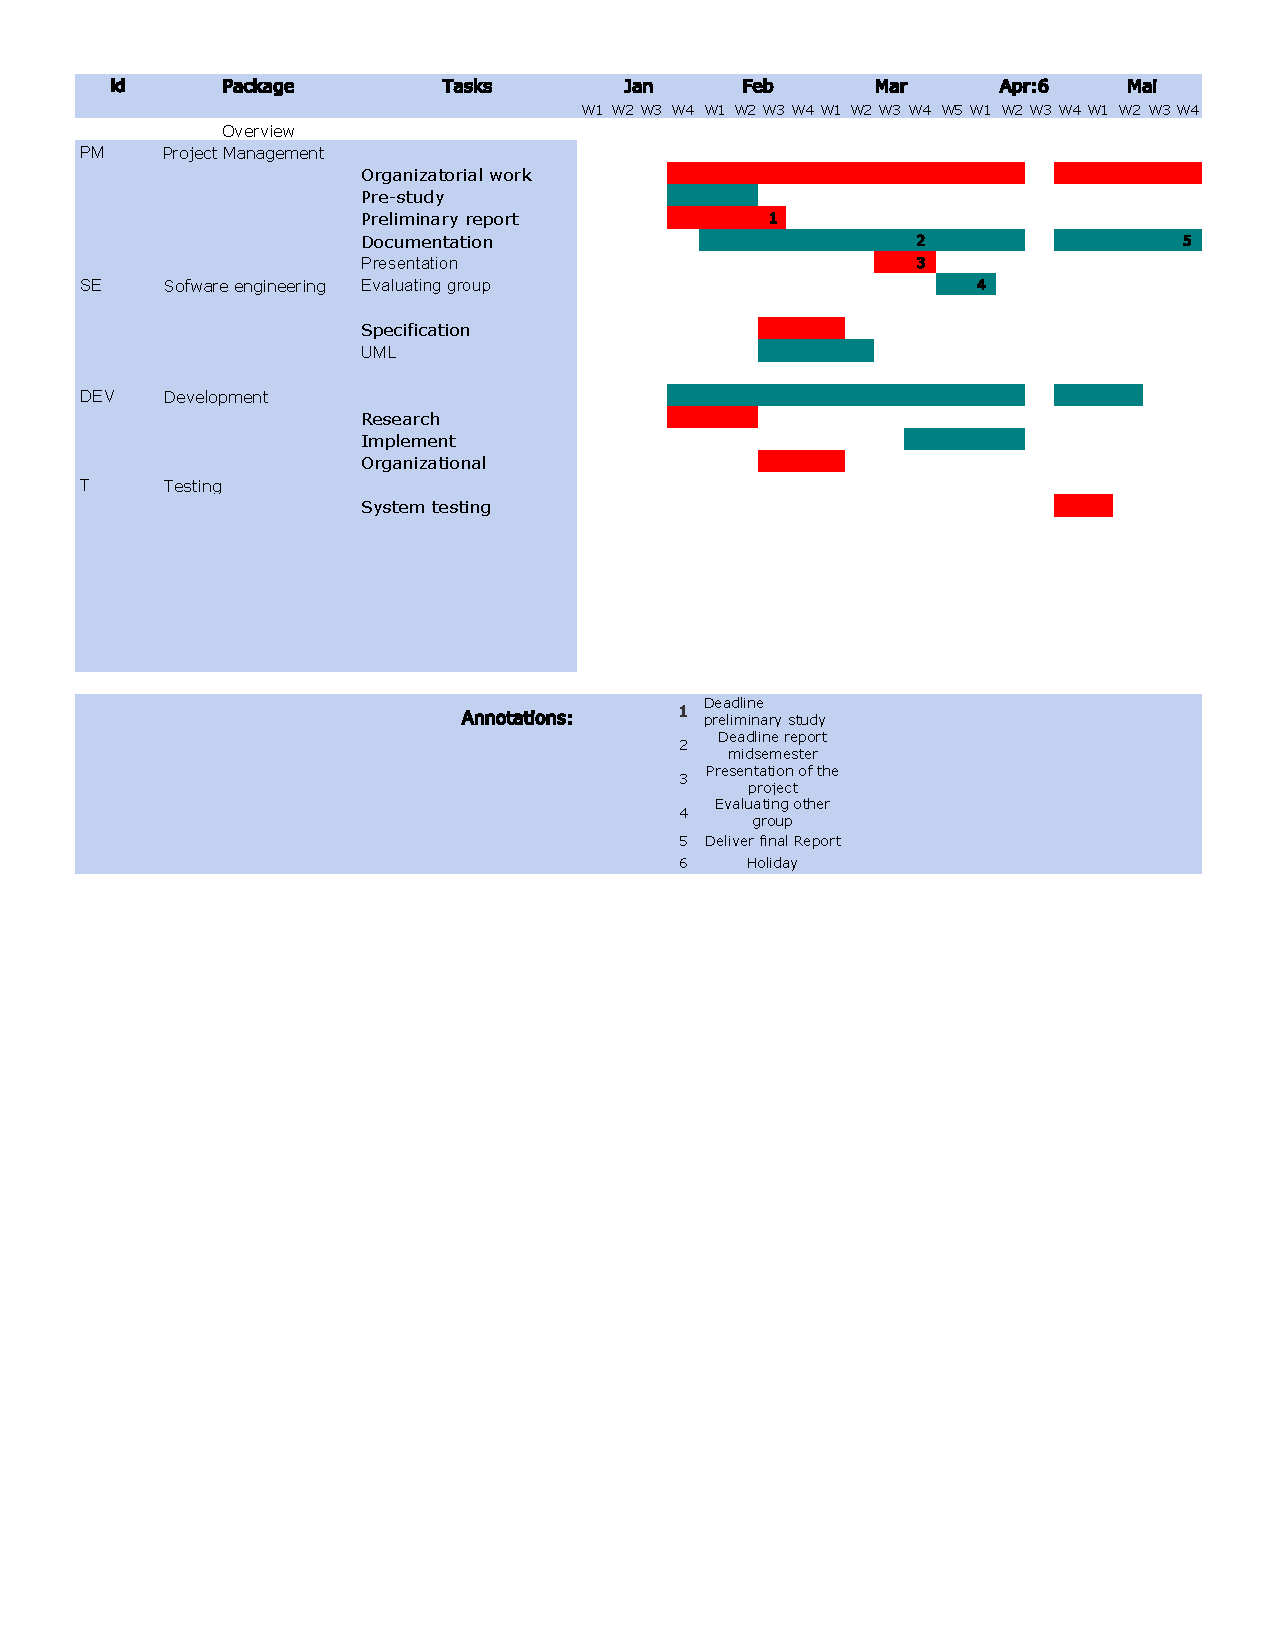
\includegraphics[keepaspectratio=true,width=\linewidth]{gantt}
					
		\section{Software Engineering}
			\subsection{Tentative architecture}
				\includegraphics[keepaspectratio=true,width=\textwidth]{architecture}
			\subsection{Requirements}
				\subsubsection{Functional Requirements}
					\paragraph{}
						
					\begin{description}
						\item[Continue developing on the existing platform] \hfill \\
						The application is developed with the Titanium SDK to maintain and continuing the development of the application ours also have to be that.
						\item[Preferably no backend] \hfill \\
						The customer does not want to maintain a backend. This also have a privacy perspective. 
						\item[Compiled multi-platform application]  \hfill \\
						As of today the application is compiled so that it can be added to Apple Store and Google Play.
						\item[Application for mobile devices]  \hfill \\
						The application is meant for smartphones and should not have a web interface.
					\end{description}			
				\subsubsection{Non-Functional Requirements}
The non-functional 
					

			\subsection{External perspective}
				\subsubsection{Activity Diagram}
(...)
			\subsection{Interactions}
				\subsubsection{Use-cases}
(...)
				\subsubsection{Sequense diagrams}
(...)
			\subsection{Structure}
				\subsubsection{Class Diagram}
(...)
			\subsection{Behavior}
				\subsubsection{State Diagram}
(...)

		\section{Implementation}
(...)
		\section{Testing}
(...)
		\section{Summary}
(...)
		\section{Conclusion}

	\printbibheading
	\printbibliography[type=book,heading=subbibliography,title={Book Sources}]
	\printbibliography[nottype=book,heading=subbibliography,title={Other Sources}]	

	\appendix
			\section{Documents}
				\subsection{Risk analysis}	
					\begin{center}
						\begin{tabulary}{\textwidth}{LRCCCLR} \toprule
Problem & Description & Likelihood (1-9) & Impact (1-9) & Importance (Likelihood * Impact) & Preventive action & Remedial Action \\ \bottomrule
						\end{tabulary}
						\begin{tabulary}{\textwidth}{LRCCCLR} \\
Communication Loss & Group members doesn't communicate with each other. Group don't establish good communication with the customer and supervisor & 3 & 7 & 21 & Actively establish communication and reach out to the parties. & Talk with the group about the communication, and try to get a good grip of what is failing. Establish communication media, so the group can talk with eachother.\\ 
\hline
Change requests & Change requests that does not meet the requirements of the product & 3 & 7 & 21 & Well defined requirements spesification, implementing it iterative. & Talk with the customer and ask what he thinks about the request changes.\\ 
\hline
Technical difficulties
 & Some problems may turn up to be very hard to solve. This can in turn lead to delays and frustration. And may sometimes be very time consuming. & 5 & 4 & 20 & Regulary have technical discussions with the group, that way the hard problems can be handled by the group as a whole.
 & If the problem is to hard, try to get help from other groups. Also evaluate if the problem can be handled differentely.\\ 
\hline
						\end{tabulary}
						\begin{tabulary}{\textwidth}{LRCCCLR} \toprule
Workstation are noisy & The workstation is filled with people who make alot of sound, so the developers team can't concentrate to the fullest. & 5 & 4 & 20 & Can preorder room, so we get our own workstation to work on. & Preorder room, and move the whole developers team there. If the noise is that bad.\\ 
\hline
Failing to do planned work & Members of the group fails to do schedueld work due to falling behind in subjects not related to the project or other things.  & 9 & 2 & 18 & Good scheduling habits. Sit down every week and see what's planned to do in the project the following week. Coordinate against what you have to do in other subject. & Make up for lost work during weekends or other available time slots\\ 
\hline
Insufficient product & Devolping a product that does not meet the requirements of the costumer & 2 & 9 & 18 & Good communication with the costumer, in sort of agile devolpment such as Scrum & \\ 
\hline
API change & The general API has to be changed, because it lack functionality. & 2 & 9 & 18 & Sufficient research about API before implementing it into the project. & Either drop the functionality that is missing, or start developing with the new API.\\ 
\hline
						\end{tabulary}
						\begin{tabulary}{\textwidth}{LRCCCLR} \toprule
Different app views & Customer and developers have different views of the apps purpose and funtions & 3 & 6 & 18 & Have regular meetings, inform and discuss all changes to project scope, goals and features. & Discuss with customer and find middle ground.\\ 
\hline
Scope & The amount of features requested are beyond what the development team can deliver in time & 6 & 3 & 18 & Be specific with the customer how much time we have, and explain deeply how much time it takes to develop a single feature & Discuss what are the nessasery features that must be in the product, and flush out what is the least nessasery.\\ 
\hline
Lack of competence & Don't have enough competence about the given software we are suppose to use during the project. & 8 & 2 & 16 & Meet every day, do workgroups together and learn by failing. & Talk with other members of the group, and hear if they have the competence. This will prevent hours of searching, when you can listen what the other members have to say. And direct you on the right path for the competence you need.\\ 
\hline
						\end{tabulary}
						\begin{tabulary}{\textwidth}{LRCCCLR} \toprule
Install of stedr & Not all group members can install the app on their own device. The purpose is to evaluate stedr. & 5 & 3 & 15 & Install it while you have a meeting, so all the group members can atleast watch the app on another device. & Go together 2 and 2, and watch the app on a phone whose able to install the app.\\ 
\hline
Missing deadlines & Some work may take longer time than expected, this this may cause delays later on in the project. & 3 & 5 & 15 & Have a steady and diciplined workflow and plan ahead. Overestimate work rather than underestimate. & All members meet and plan what is to be done, and do it at once. So we can deliver as soon as possible.\\ 
\hline
Customer turnover disruption & A key contact in SINTEF leaves the company, putting the project in a unclear state & 2 & 7 & 14 & Good communication. Multiple contacts with knowledge of the project & Quickly contact the customer and discuss how to proceed and how it's affected\\ 
\hline
Sickness & Group members or other crucial personell gets sick & 4 & 3 & 12 & Have regular updates about the progress of the work being done, and don't make important task rely completely on one person without a backup plan. Don't freeze and drink a lot of tea. & Talk to the person about the individual tasks, how much he can handle, and distribute the work the member can't.\\ 
\hline
						\end{tabulary}
						\begin{tabulary}{\textwidth}{LRCCCLR} \toprule
Group members falling out. & Members doesn't show for meetings, or goes of the grid without notice. & 2 & 6 & 12 & Good communication and agree on a schedule that suits everyone. & Take action at once, and make inquires to why the member didn't show.\\ 
\hline
Uneven workload & Uneven distribution of workload & 6 & 2 & 12 & Keep updated on the tasks given and work put in, and distribute work  & Make the member or members direct task. So it's easy for the member or members to do so. \\ 
\hline
Conflict over changes & Group members not in agreement over supposed changes in group management, work, responibility etc. & 3 & 4 & 12 & Have an open dialog. & Discuss in group and decide as a democracy.\\ 
\hline
Late for meeting & Members of the group are late for meetings with group/customer and supervisor & 6 & 2 & 12 & Good communication and agree on a schedule that suits everyone. & Take action at once, and make inquires to why the member came late.\\ 
\hline 
						\end{tabulary}
						\begin{tabulary}{\textwidth}{LRCCCLR} \toprule
Documents customer/supervisor meeting & You lack the sufficeint documents for the meeting with the customer. For presentation on how you want the app to be, mockups and reports about fieldwork etc. & 2 & 6 & 12 & Have the documents stored in the cloud so  you can acces it where ever you go. With your respective smartphone/tablet and pc's, & Discuss what you remember and try to make the best out of the meeting, as possible.\\ 
\hline
Equipment failure & Computers and other dependable devices malfunctions. & 4 & 2 & 12 & Keep documents and code in the cloud so you can work from another device if your primary device malfunction. & Get replacement as soon as possible.\\ 
\hline
Document sharing failed & Authorization of documents sharing is not complete, people don't have access to the groups documents. & 2 & 4 & 8 & Give all the authorization they need for the documents to be shared. So all can view, edit and share documents. & Find out where the problem lies, so everyone can get authorization for the given documents and folders.\\ 
\hline
						\end{tabulary}
						\begin{tabulary}{\textwidth}{LRCCCLR} \toprule
Lack of software  & nessasery for the develoment progress & 1 & 3 & 3 & Talk about what software is required for the development of the product. Ask the customer for this software.   & Ask the customer immediately for the required software, so the development progress don't have any major delays. \\ 
\hline

						\end{tabulary}
					\end{center}



\end{document}